% Abstract for this chapter
%
%**********************************************************************
% Under the inspection task,
% despite the reaction wheels can compensate the base disturbance induced by the manipulator motions
% because that is not so large especially as shown in \fig{RES_INS2},
% we will show that the reaction wheels have a disadvantage in terms of energy consumption.

So far, reaction wheels have been used to stabilize the base attitude against
the base reaction induced by a manipulator motion.
However, as explained in \cha{INTRO},
the output torque of reaction wheels are far smaller than the base reaction.
In addition to this problem,
it is known that reaction wheels need a large amount of energy 
if a large output torque is produced \cite{Carpenter2009}.
On the other hand,
reactionless motion control need not use reaction wheels.
Hence, we can expect that energy consumption during a task can be reduced through reactionless motion control.
In fact,
we will show that reactionless motion coincides with the instantaneous minimum energy motion.
% In this chapter,
% we treat the energy consumption of reaction compensation.
% First, we identify the minimum energy motion under zero 
% base-attitude deviation ($\bm{\omega}_{b} \approx \bm{0}$) and
% show that it is almost equivalent to reactionless motion control.
% This character arises from, under reactionless motion control, 
% the no usage of reaction wheels and its high amount of energy consumption.
% Note that we restrict our attention to the system which consists of
% one manipulator and three reaction wheels, for the sake of simplicity.

%%%%%%%%%%%%%%%%%%%%%%%%%%%%%%%%%%%%%%%%%%%%%%%%%%%%%%%%%%%%%%%%%%%%%%%%%
\section{Kinetic energy}
%%%%%%%%%%%%%%%%%%%%%%%%%%%%%%%%%%%%%%%%%%%%%%%%%%%%%%%%%%%%%%%%%%%%%%%%%
In this work, we assume that kinetic energy is used to evaluate energy consumption.
For the sake of simplicity,
we ignore energy losses arising from friction, heat and the electric parts.
The kinetic energy of the space robot system can be written as \cite{Masutani,Dimitrov2004}:
%
% ---------------------------------------------------------------------
\begin{align}
  T = \frac{1}{2}\bm{\omega}_{b}^{T}\tbm{M}_{\omega}\bm{\omega}_{b} +
  \bm{\omega}_{b}^{T}\bmat{\tbm{M}_{\omega m} & \tbm{M}_{\omega r}}\bmat{\thd \\ \phd}
  + \frac{1}{2}\bmat{\thd^{T} & \phd^{T}}\bmat{\tbm{M}_{m} & \bm{0} \\ \bm{0} & \tbm{M}_{r}}\bmat{\thd \\ \phd}\label{eq:kin1}
\end{align}
% ---------------------------------------------------------------------
%
where the first term on the r.h.s.\ represents the partial kinetic energy stemming from base rotation,
the second term is the coupling kinetic energy between the base and the manipulator or the reaction wheels.
Finally,
the third term is the partial kinetic energy produced by the manipulator and the reaction wheels.

With the assumption $\bm{\omega}_{b} \approx \bm{0}$, \eq{kin1}  simplifies as:
%
% ---------------------------------------------------------------------
\begin{align}
  T = \frac{1}{2}\thd^{T}\tbm{M}_{m}\thd + \frac{1}{2}\phd^{T}\tbm{M}_{r}\phd.
\label{eq:kin2}
\end{align}
% ---------------------------------------------------------------------
%
Further on, from angular momentum conservation,
the reaction wheel speed can be represented as a function of the joint velocity,
$\phd = -\tbm{M}_{\omega r}^{-1}\tbm{M}_{\omega m}\thd$.
Substitute this expression  into \eq{kin2} 
to obtain the kinetic energy as a function of the joint velocity:
%
% ---------------------------------------------------------------------
\begin{align}
  T &= \frac{1}{2}\thd^{T}\Big(\tbm{M}_{m} + 
  \tbm{M}_{\omega m}^{T}(\tbm{M}_{\omega r}\tbm{M}_{r}^{-1}\tbm{M}_{\omega r}^{T})^{-1}\tbm{M}_{\omega m}\Big)\thd \notag\\
  &= \frac{1}{2}\thd^{T}\Big(\tbm{M}_{m} + I_{r}^{-1}\tbm{M}_{\omega m}^{T}\tbm{M}_{\omega m}\Big)\thd \notag\\
  &= \frac{1}{2}\thd^{T}\bm{\Lambda}\thd\label{eq:kin}
\end{align}
% ---------------------------------------------------------------------
%
where $\bm{\Lambda} = \bm{\Lambda}_{m} + \bm{\Lambda}_{r}$ is the inertia matrix of the manipulator
under zero attitude deviation. Matrices 
$\bm{\Lambda}_{m} = \tbm{M}_{m}$ and
$\bm{\Lambda}_{r} = I_{r}^{-1}\tbm{M}_{\omega m}^{T}\tbm{M}_{\omega m}\R{n \times n}$ are
inertias associated with the manipulator and the reaction wheels, respectively.
In the above derivation,  we assume that $\tbm{M}_{\omega r} \approx \tbm{M}_{r}$.
Also it is assumed that the reaction wheels are located on mutually orthogonal axes 
for zero-momentum stabilization and that  $\tbm{M}_{r} = \mathrm{diag}(I_{r},I_{r},I_{r})$.

Further on, the direction of instantaneous minimum energy motion can be obtained through SVD of
 matrix $\bm{\Lambda}$ \cite{Torres1993}:
%
% ---------------------------------------------------------------------
\begin{align}
  \bm{\Lambda} = \sigma_{1}\bm{u}_{1}\bm{v}_{1}^{T} + \sigma_{2}\bm{u}_{2}\bm{v}_{2}^{T} 
     + \cdots + \sigma_{n}\bm{u}_{n}\bm{v}_{n}^{T}
  \label{eq:svd}
\end{align}
% ---------------------------------------------------------------------
%
where  $\sigma_{i}~(\sigma_{1} \geq \sigma_{2} \geq \cdots \geq \sigma_{n})$ are the singular values.
%and $\bm{u}_{i}$ and $\bm{v}_{i}$ denote the left and right singular vectors.
The meaning of the right singular vectors, $\bm{v}_{i}$, can be interpreted as normalized 
joint velocity, while that of singular value $\sigma_{i}$ as kinetic energy induced 
by  joint motion $\bm{v}_{i}$. Then, $\sigma_{n}$ represents the instantaneous minimum 
kinetic energy, while $\bm{v}_{n}^{T}$ determines the minimum energy motion direction.

%%%%%%%%%%%%%%%%%%%%%%%%%%%%%%%%%%%%
\section{Motion equivalence}
%%%%%%%%%%%%%%%%%%%%%%%%%%%%%%%%%%%%
Here, we compare reactionless motion and the instantaneous minimum energy motion via numerical analysis.
For the sake of simplicity, we  focus on models comprising only one-DoF reactionless motion.

%%%%%%%%%%%%%%%%%%%%%%%%%%%%%%%%%%%%%%%%%%%%%%%%%%%%
\subsubsection{Two-DoF planar manipulator}
%%%%%%%%%%%%%%%%%%%%%%%%%%%%%%%%%%%%%%%%%%%%%%%%%%%%
%
First, a two-DoF planar model is considered, as shown in \fig{FF2R}.
The link lengths, masses and inertia moments are set to $l_{i} = 1.0\unit{m}$,
$m_{i} = 100\unit{kg}$ and $I_{i} = 8.3\unit{kgm^{2}}~(i=1,2)$, respectively.
The reaction wheel's mass and inertia moment are set to $m_{r} = 10\unit{kg}$,
$I_{r} = 0.11\unit{kgm^{2}}$.
The manipulator attachment position is defined as $r = 0.945\unit{m}$ and $\psi = 0\unit{rad}$.

The following cost function will be used to evaluate the energy relation for 
reactionless motion and instantaneous minimum energy motion:
% %
% % ---------------------------------------------------------------------
% \begin{align}
%   C_{err} = \tan^{-1}\Big(\frac{\sqrt{1 - |\thd_{min}^{T}\thd_{rlm}|^{2}}}{|\thd_{min}^{T}\thd_{rlm}|}\Big)\unit{[rad]}
% \end{align}
% % ---------------------------------------------------------------------
% %
%
% ---------------------------------------------------------------------
\begin{align}
  C_{ratio} = \frac{T_{RNS}}{T_{min}}.
\end{align}
% ---------------------------------------------------------------------
%
 $T_{RNS}$ and $T_{min}$ denote the  kinetic energies under
reactionless  and  instantaneous minimum energy motion, respectively.
Because $T_{RNS} \geq T_{min}$ at all configurations, $C_{ratio} \geq 1$ is ensured.
%$C_{ratio}$ takes close to 1 means these motion are equivalent.
This function will be calculated at a mesh of 10K points in joint space, 
with $-\pi \leq \theta_{i} \leq \pi$, $(i = 1,2)$.
For each coordinate, the joint angles are discretized with $\Delta \theta_{i} = 6.28\times 10^{-2}\unit{rad}$.

According to \eq{svd}, $\thd_{min}$ can be obtained as $\bm{v}_{2}$ and reactionless motion
is obtained through SVD of the coupling inertia matrix.
The distribution of $C_{ratio}$ is displayed in \fig{dist_2D}.
%
% ---------------------------------------------------------------------
\begin{figure}[t]
  \centering
  \begin{minipage}{0.49\linewidth}
    \centering
    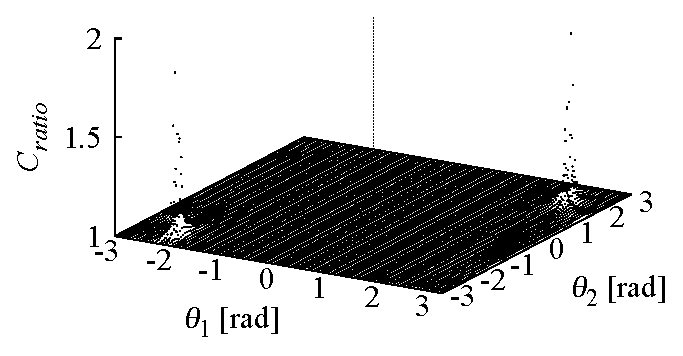
\includegraphics[width=1.0\linewidth]{fig/chapter5/analysis/err.eps}
  \end{minipage}
  \begin{minipage}{0.37\linewidth}
    \centering
    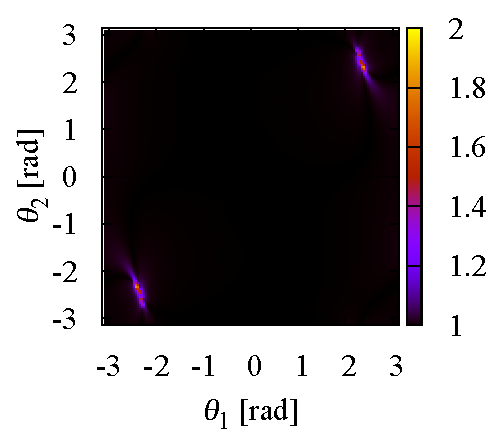
\includegraphics[width=1.0\linewidth]{fig/chapter5/analysis/err_2d.eps}
  \end{minipage}
  \caption{The distribution of the cost function with the two-DoF model.}
  \label{fig:dist_2D}
\end{figure}
% ---------------------------------------------------------------------
%
From the result,
we can confirm that $C_{ratio} \approx 1$ at almost all points.
Indeed, the average of $C_{ratio}$ is $1.002$  among all points.
Hence, these motions are equivalent with this model.
Here, we should note that there are large errors at specific points.
This non-correspondence will be discussed below.


%%%%%%%%%%%%%%%%%%%%%%%%%%%%%%%%%%%%%%%%%%%%%%%%%%%%%%%%%%
\subsubsection{The role of parameter variation}
%%%%%%%%%%%%%%%%%%%%%%%%%%%%%%%%%%%%%%%%%%%%%%%%%%%%%%%%%%
Before examining the energy ratio with a  spatial model,
we should identify the influence arising from parameter variation.
Here, we focus on variations of the mass and the CoM position of each link according 
to the following equations:
%
% ---------------------------------------------------------------------
\begin{align}
  m_{i}^{*} &= \alpha m_{i}\\
  l^{*}_{ci} &= \beta l_{ci}
\end{align}
% ---------------------------------------------------------------------
%
where  $0.5 \leq \alpha \leq 1.5$,
$0.5 \leq \beta \leq 1.5$  are the variation factors and 
$l_{ci} = l_{i}/2$ denotes  the CoM position of each link.
% as explained above ($m_{i} = 100\unit{kg}$, $l_{i} = 1\unit{m}$).
%$(\circ)^{*}$ denotes the modified parameter.
%
% ---------------------------------------------------------------------
\begin{figure}[t]
  \centering
  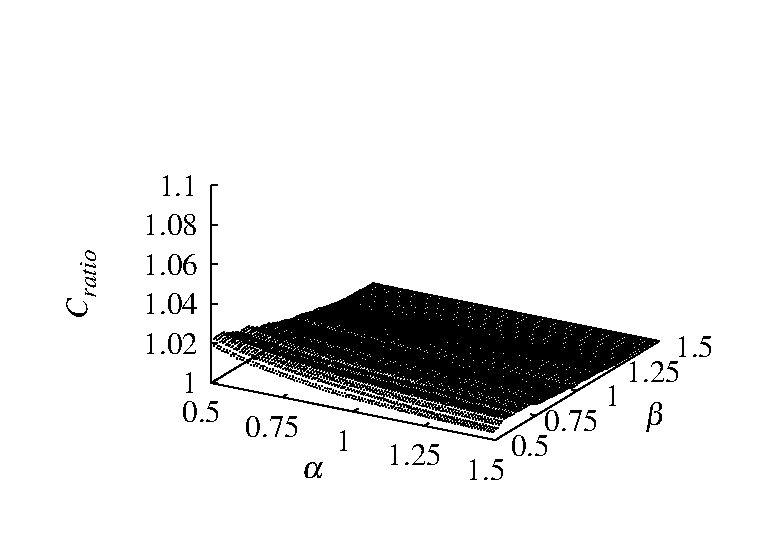
\includegraphics[width=0.6\linewidth]{fig/chapter5/analysis/parameter.eps}
  \vspace{-2em}
  \caption{This figure shows how the average of $C_{ratio}$ is affected by parameter variation.}
  \label{fig:parameter}
\end{figure}
% ---------------------------------------------------------------------
%
The average of $C_{ratio}$ under such variations is displayed in \fig{parameter}.
This figure shows that reactionless motion approximately coincides
with instantaneous minimum motion even if the parameters are varied.
In particular, high equivalence can be observed when $\alpha$ takes large values.

%%%%%%%%%%%%%%%%%%%%%%%%%%%%%%%%%%%%%%%%%%%%%%%%%%%%
\subsubsection{Four-DoF spatial manipulator}
%%%%%%%%%%%%%%%%%%%%%%%%%%%%%%%%%%%%%%%%%%%%%%%%%%%%
The positioning subchain of the seven-DoF redundant manipulator introduced in \sec{MODEL}
will be used to evaluate the energy ratio.
The reaction wheel parameters are the same as in the planar case.
The same cost function is also used to evaluate the equivalence.
The calculation range is as follows:
%
% ---------------------------------------------------------------------
\begin{align}
  &-\pi \leq \theta_{i} \leq \pi\notag\\
  &\Delta \theta_{i} = 0.125\unit{rad}~(i = 1,3,4)\\
  &-\frac{\pi}{2} \leq \theta_{2} \leq \frac{\pi}{2}\notag\\
  &\Delta \theta_{2} = 0.0628\unit{rad}
\end{align}
% ---------------------------------------------------------------------
%
where  we restrict the range of Joint 2 because almost all configurations outside 
the above range have no meaning due to the collision with the satellite.
The cost function is calculated at $6.25\times 10^{6}$ points.

Because of the number of parameters is large, 
we show the distribution of $C_{ratio}$ parametrized for Joint 1 and 2.
First, in \fig{dist_3d}~(a)  a distribution map is shown that  does not include large errors. 
The map was obtained with the parametrization $(\theta_{1}, \theta_{2}) = (-3.05,0.403)\unit{rad}$.
Except few configurations, 
reactionless motion coincides with the energy minimum motion, as  in the planar case.
However, we observe some inconsistency at specific configurations.
An example is shown in \fig{dist_3d}~(b) with the parametrization $(\theta_{1},\theta_{2}) = (-\pi,0)\unit{rad}$.
Despite these large errors, the average value of $C_{ratio}$ is $1.14$.
Hence, it can be concluded that reactionless motion produces approximately minimum energy motion.
In what follows, we discuss the reasoning behind this observation and the cases of inconsistency.
%
% ---------------------------------------------------------------------
\begin{figure}[t]
  \centering
  \begin{minipage}[t]{0.495\linewidth}
    \centering
    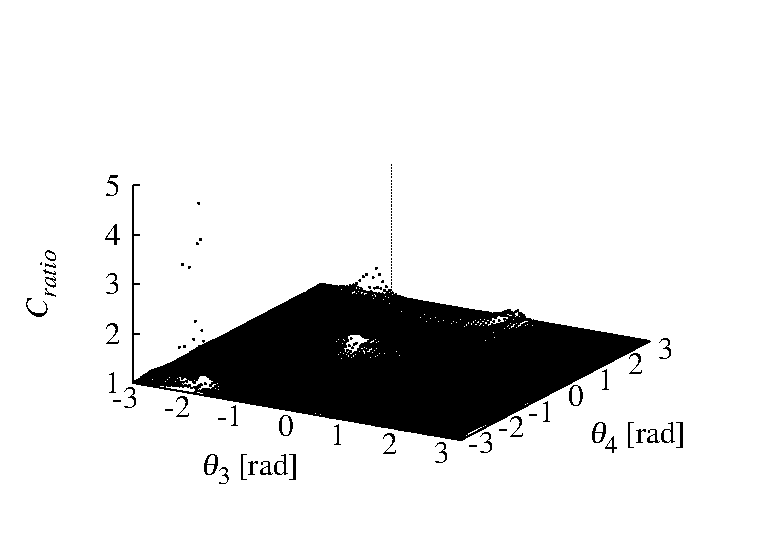
\includegraphics[width=1.0\linewidth]{fig/chapter5/analysis/err-3.05183_0.403919.eps}
    \footnotesize\par{(a)}
  \end{minipage}
  \begin{minipage}[t]{0.495\linewidth}
    \centering
    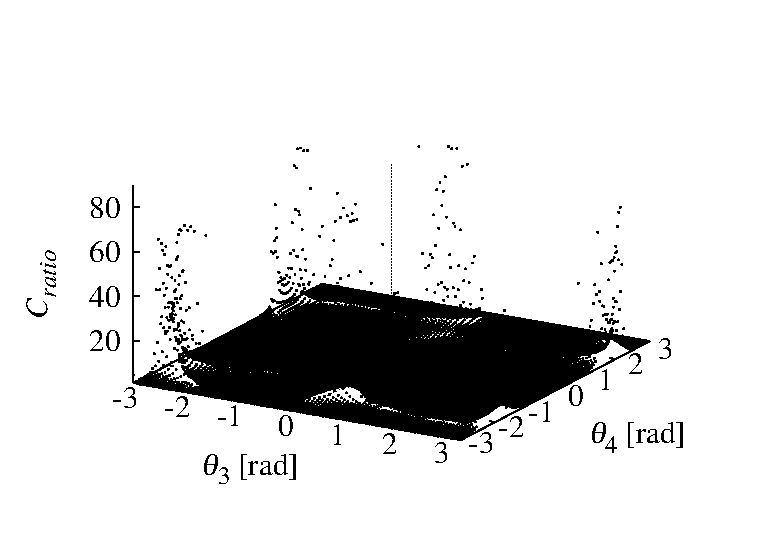
\includegraphics[width=1.0\linewidth]{fig/chapter5/analysis/err-3.14159_0.eps}
    \footnotesize\par{(b)}
  \end{minipage}
  \caption{The disutribution of cost function with the four-DoF spatial manipulator model:
  (a) regularly appearing distribution $(\theta_{1},\theta_{2}) = (-3.05,0.403)\unit{rad}$
  and (b) near the singularity $(\theta_{1},\theta_{2}) = (-\pi,0)\unit{rad}$.}
\label{fig:dist_3d}
\end{figure}
% ---------------------------------------------------------------------
%

%%%%%%%%%%%%%%%%%%%%%%%%%%%%%%%%%%%%%%%%%%%%%%%%%%%%%%%%%%%%%%
\subsubsection{Discussion}% about the equivalence}
\label{sec:DISCUSS}
%%%%%%%%%%%%%%%%%%%%%%%%%%%%%%%%%%%%%%%%%%%%%%%%%%%%%%%%%%%%%%
%
To reason about the equivalence, we should identify a property of kinetic energy 
produced by both manipulator and reaction wheels under zero base-attitude deviation.
This property appears in the inertia matrix.
$\bm{\Lambda}_{m}$ and
$\bm{\Lambda}_{r}$ are rewritten in the following form:
%
% ---------------------------------------------------------------------
\begin{align}
  \bm{\Lambda}_{m} = &\sum_{i=1}^{n}\Big\{m_{i}\bm{J}_{vi}^{T}\bm{J}_{vi} + \bm{J}_{\omega i}^{T}\bm{I}_{i}\bm{J}_{\omega i}\Big\}\label{eq:mani}\\
  \bm{\Lambda}_{r} = &\frac{1}{I_{r}}\sum_{i=1}^{n}\Big\{m_{i}^{2}\bm{J}_{v i}^{T}[\bm{r}_{b \rightarrow i}^{\times}]^{T}[\bm{r}_{b \rightarrow i}^{\times}]\bm{J}_{vi}+
\bm{J}^{T}_{\omega i}\bm{I}_{i}\bm{I}_{i}\bm{J}_{\omega i} +\notag\\
  &m_{i}\bm{J}_{\omega i}^{T}\bm{I}_{i}[\bm{r}_{b \rightarrow i}^{\times}]\bm{J}_{vi} + [ m_{i}\bm{J}_{\omega i}^{T}\bm{I}_{i}[\bm{r}_{b \rightarrow i}^{\times}]\bm{J}_{vi}]^{T}\Big\}\label{eq:rw}
\end{align}
% ---------------------------------------------------------------------
%
where  $m_{i}$, $\bm{I}_{i}\R{3}$ are $i$-th link mass and inertia tensor,
$\bm{J}_{vi}$,
$\bm{J}_{\omega i}\R{3 \times n}$ stand for the Jacobian w.r.t.\ linear and angular velocity of each link,
$\bm{r}_{b \rightarrow i}\R{3}$ is the position vector of the $i$-th link CoM w.r.t.\ the base CoM.
Here, we assume a general $n$-link manipulator model.
Note that terms related to base translation are ignored for the sake of simplicity.

From \eq{mani}, it can be seen that the kinetic energy induced by the manipulator motion is represented
as a linear function in terms of the inertia parameters of manipulator.
On the other hand, the
reaction wheel related energy is a quadratic function of the same parameters;
it is also in proportion to the inverse of the inertia moment of the reaction wheel,
which is usually much smaller than 1.
Hence, we can conclude that the  kinetic energy produced by the reaction wheels 
is much larger than that by the manipulator. 
This feature would make reactionless motion potentially effective in terms of energy consumption 
because the usage of reaction wheels can be avoided.

On the other hand, comparing the results in \fig{BIF_VEC}~(b) and \fig{dist_2D},
we can find that there is some  inconsistency around the singularities of the coupling 
inertia matrix. In particular, at such a singularity,
any motion would not disturb the base attitude because the dimension of the null-space of the 
coupling inertia matrix increases. A second reactionless motion vector appears then 
at the singularity and both null-space vectors span the  tangent space of joint 
space $T_{\theta}(\mathbb{R}^{2})$. This means that reactionless motion must be at 
the energy minimum. On the other hand,
near a singularity, reactionless motion deviates from the instantaneous energy 
minimum motion.
At these configurations, because the base disturbance is minute,
a large effort of the reaction wheels is hardly needed.
Namely, the kinetic energy stemming from the reaction wheels becomes small,
and hence a manipulator motion whose kinetic energy is minimum or at least smaller than
that reactionless motion induces can be closer to the minimum energy motion than reactionless motion be.


%%%%%%%%%%%%%%%%%%%%%%%%%%%%%%%%%%%%%%%%%%%%%%%%
\subsection{Comparative  study for the inspection task}
\label{sec:comp}
%%%%%%%%%%%%%%%%%%%%%%%%%%%%%%%%%%%%%%%%%%%%%%%%

%%%%%%%%%%%%%%%%%%%%%%%%%%%%%%%%%%%%%
\subsubsection{Simulation condition}
%%%%%%%%%%%%%%%%%%%%%%%%%%%%%%%%%%%%%
%
We evaluate the performance of reactionless motion control in terms of energy consumption
during the inspection maneuver.
From the above analysis it became apparent that reactionless motion produces nearly 
 minimum energy motion and that the use of reaction wheels would be inefficient from the 
viewpoint of energy consumption, when  compensating base disturbance.

We consider the following cost functions to evaluate the performance:
%
% ---------------------------------------------------------------------
\begin{align}
  C_{max} &= \frac{1}{2}\max_{t_{0} \leq t \leq t_{f}}\Big(\thd^{T}(t)\bm{\Lambda}\thd(t)\Big)
\label{eq:Tmax}\\
  C_{sum} &= \frac{1}{2}\int_{t_{0}}^{t_{f}}\thd^{T}(t)\bm{\Lambda}\thd(t)dt.
\label{eq:Tsum}
\end{align}
% ---------------------------------------------------------------------
%
% \eq{Tmax} is the maximum kinetic energy,
% \eq{Tsum} expresses the whole kinetic energy throughout the motion tasks.
In order to realize zero base-attitude deviation with the reaction wheels,
the reaction wheel torque should be:
%
% ---------------------------------------------------------------------
\begin{align}
  \bm{\tau}_{r}^{ref} = -\frac{d}{dt}(\tbm{M}_{\omega m}\thd^{ref}(t))
\end{align}
% ---------------------------------------------------------------------
%
where $\thd^{ref}$ is the pre-defined reference control command for the manipulator.
We compare the above costs under the camera inspection task under five conditions
with different  initial configurations and desired motions.
In  all cases, the simulation time is set at $20\unit{s}$ and the comparison controller is
the inverse Jacobian controller using only the wrist assembly, as explained in the previous section.


%%%%%%%%%%%%%%%%%%%%%%%%%%%%%%%%%%
\subsection{Simulation results}
%%%%%%%%%%%%%%%%%%%%%%%%%%%%%%%%%%
%
% ---------------------------------------------------------------------
\begin{figure}[t]
  \centering
  \begin{minipage}[h]{0.5\linewidth}
    \centering
    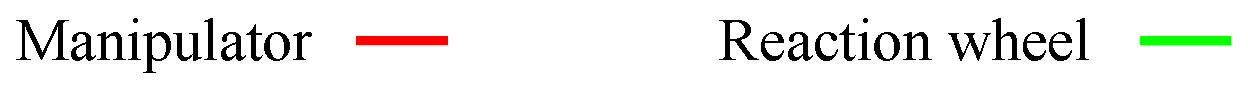
\includegraphics[width=1.0\linewidth]{fig/chapter5/comparison/energy.eps}
  \end{minipage}\\
  \vspace{-4mm}
  \begin{minipage}[h]{0.40\linewidth}
    \centering
    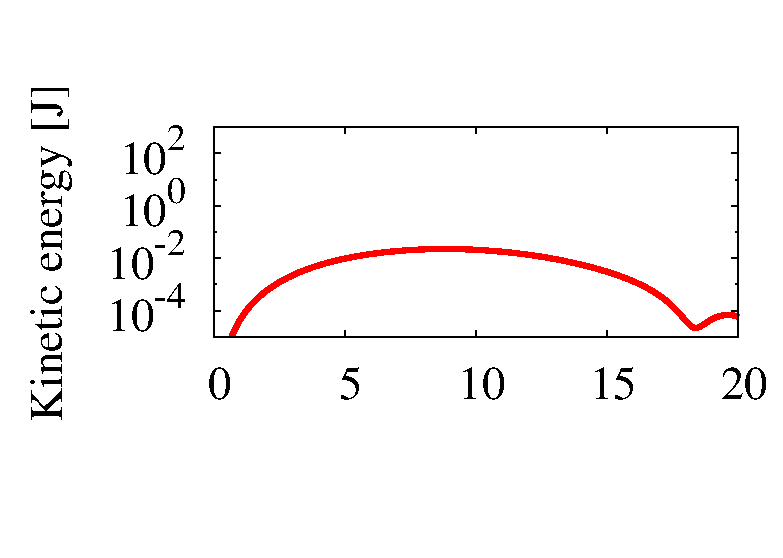
\includegraphics[width=1.0\linewidth]{fig/chapter5/comparison/RL-M/RNS_U10_partial_kinetic_energy.eps}
  \end{minipage}
  \hspace{-4mm}
  \begin{minipage}[h]{0.40\linewidth}
    \centering
    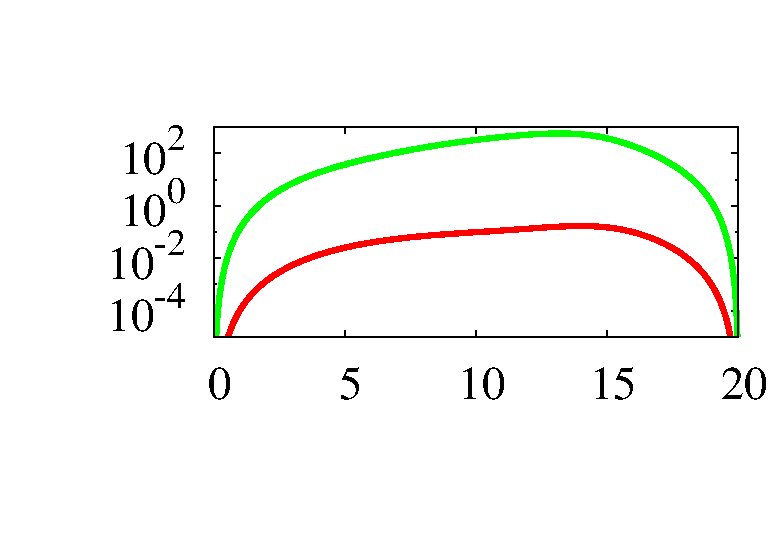
\includegraphics[width=1.0\linewidth]{fig/chapter5/comparison/RW-M/RNS_U10_partial_kinetic_energy.eps}
  \end{minipage}\\
  \vspace{-7mm}
  \centering
  \begin{minipage}[h]{0.350\linewidth}
    \centering
    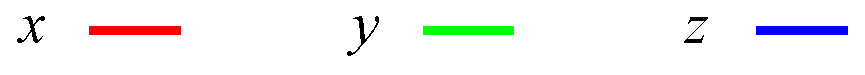
\includegraphics[width=1.0\linewidth]{fig/chapter5/comparison/torque.eps}
  \end{minipage}\\
  \vspace{-4mm}
  \begin{minipage}[h]{0.40\linewidth}
    \centering
    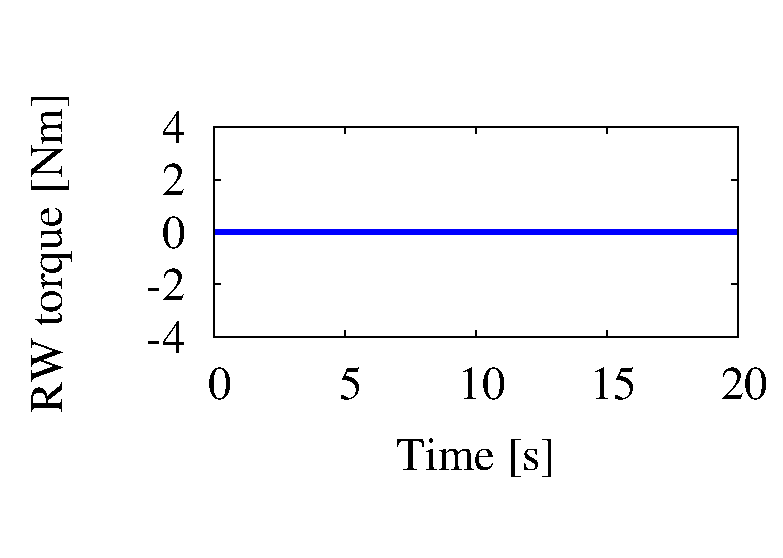
\includegraphics[width=1.0\linewidth]{fig/chapter5/comparison/RL-M/RNS_U03_reaction_wheel_torque.eps}
    \footnotesize\par{\vspace{-2mm}\hspace{8mm}Reactionless}
  \end{minipage}
  \hspace{-4mm}
  \begin{minipage}[h]{0.40\linewidth}
    \centering
    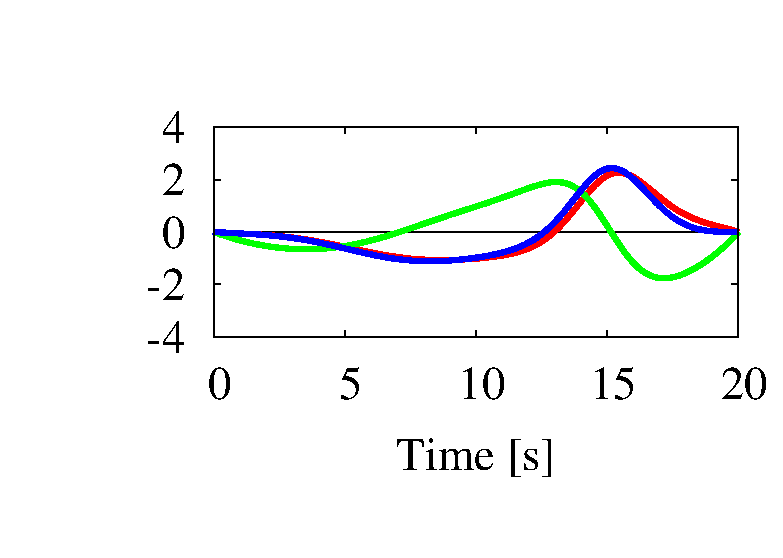
\includegraphics[width=1.0\linewidth]{fig/chapter5/comparison/RW-M/RNS_U03_reaction_wheel_torque.eps}
    \footnotesize\par{\vspace{-2mm}\hspace{8mm}Reaction wheel used}
  \end{minipage}\\
  \vspace{-4mm}
  \vspace{1em}
  \caption{An example of energy consumption comparison.}
  \label{fig:RES_ENE}
\end{figure}
% ---------------------------------------------------------------------
%
First, as an example, consider the conditions used in \sec{INSPECTION} (the case of \fig{ins}~(a)):
the initial configuration is set to $[-90~-30~0~-70~180~-30~0]^{T}\unit{deg}$,
the reference angular velocity is $\bm{\omega}_{e}^{ref} = \pi[s(t)~0~0]^{T}$,
where $0 \leq s(t) \leq 1$ denotes a fifth-order spline function;
the simulation time and the gain are set at $20\unit{s}$ and $k_{g} = 100  \unit{kg/(m \cdot s)}$, respectively.
The results are displayed in \fig{RES_ENE}.
We can see that the kinetic energy produced by the reaction wheels is quite larger than
that by the manipulator motion. Hence, in this case, we can confirm that reactionless motion 
control has an advantage in terms of energy consumption, as described above.
In addition,
if we plan to perform this inspection task with reaction wheels,
the manipulator has to be driven at lower speed because the limitation of the reaction wheel torque
is in general quite low. For instance, in the ETS-VII experiment it was  $0.1\unit{Nm}$.

Next we compare the cost for five different initial configurations and desired motions 
chosen randomly. The results are displayed  in \fig{RES_ENE_COMP}.
The red bar expresses the results under reactionless motion control;
the green bar shows the results when reaction wheels are used.
Note that vertical  axis  represents the cost in logarithmic scale.
From the results it can be seen that energy consumption under reactionless motion 
is quite smaller than that with reaction wheels.
Actually, almost $10^{3}$ times reduction is observed in each cost function.
This result stems from the large energy consumption of the reaction wheels, as explained in \eq{rw}.
In summary, we can conclude that under reactionless motion control it is possible to reduce
both, energy consumption as well as the duration of the mission.
%
% ---------------------------------------------------------------------
\begin{figure}[t]
  \centering
  \begin{minipage}[t]{0.47\linewidth}
    \centering
    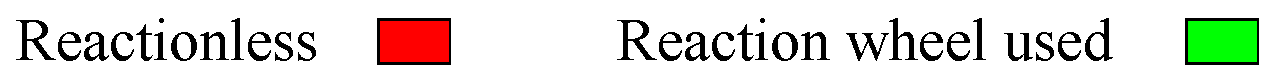
\includegraphics[width=1.0\linewidth]{fig/chapter5/comparison/comp.eps}
  \end{minipage}\\
  \vspace{-2mm}
  \begin{minipage}[t]{0.45\linewidth}
    \centering
    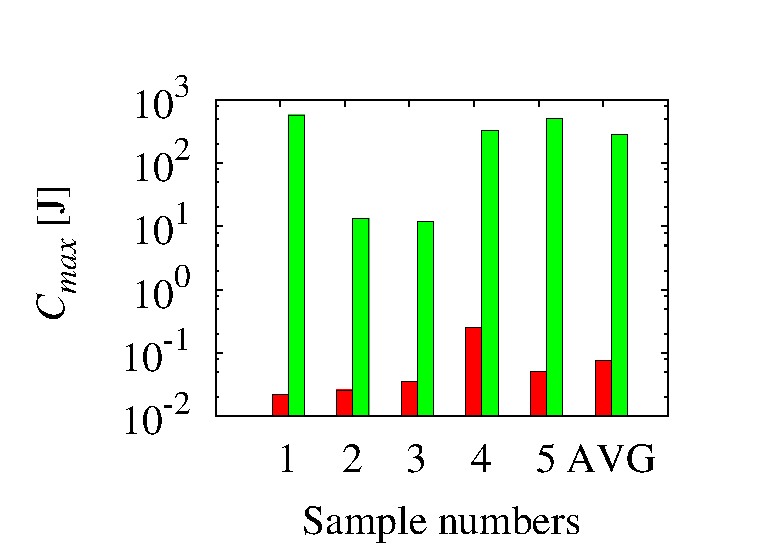
\includegraphics[width=1.0\linewidth]{fig/chapter5/comparison/01_maximum.eps}
  \end{minipage}
  \hspace{-4mm}
  \begin{minipage}[t]{0.45\linewidth}
    \centering
    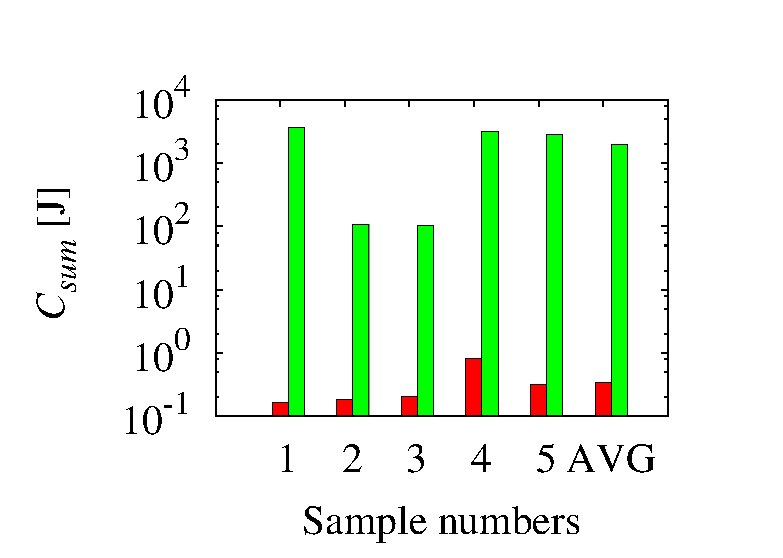
\includegraphics[width=1.0\linewidth]{fig/chapter5/comparison/02_integral.eps}
  \end{minipage}
  \caption{Comparison of energy consumption under five conditions}
  \label{fig:RES_ENE_COMP}
\end{figure}
% ---------------------------------------------------------------------
%


%%%%%%%%%%%%%%%%%%%%%
\section{Summary}
%%%%%%%%%%%%%%%%%%%%%
In this chapter, we discussed the energy consumption under zero attitude deviation.
We formulated the kinetic energy of a free-floating space robot in terms of
joint velocity under zero attitude deviation.
From the result,
we confirmed that the kinetic energy stemming from the reaction wheels is represented
as a quadratic function of the inertia parameters of the manipulator
and position vector positioning to the each line CoM,
while the kinetic energy of the manipulator is a linear function of the both quantities.
Hence, the energy consumption of the reaction wheels must be much larger than that of the manipulator.
This feature makes reactionless motion control effectiveness in terms of energy consumption.
In fact, through numerical verification,
we showed that reactionless motion coincides with the instantaneous minimum energy motion.
We compared the energy consumption of reactionless motion control with that of using reaction wheels
during some inspection tasks that was proposed in \cha{PROPOSAL}.
We obtained an interesting result that the kinetic energy during reactionless motions task
is $10^{3}$ times smaller than that during reaction wheel used task, on average.
In summary,
we can conclude that reactionless motion control has an advantage
with respect to energy efficiency.






%**********************************************************************
%
%
%%% Local Variables:
%%% mode: latex
%%% TeX-master: "./main"
%%% End: